\chapter{النموذج المقترح}

سنتكلم في هذا الفصل عن خوارزميات الملاحقة التي اعتمدنا عليها بشكل أساسي في بحثنا وهي خوارزمية 
\textLR{SwinTrack \cite{swinTrack}}
\ref{section:swintrack}
التي تعتمد على محول 
\textLR{Swin \cite{swintransformer}}
كـ
\textLR{backbone}،
وتستخدم بنية مرمز - مفكك ترميز
%\textLR{encoder-decoder}
بتوابع انتباه متعدد الرؤوس 
\textLR{MHA}.
مشكلة هذه الخوارزمية أنها تستخدم المعلومات المكانية (معلومات المظهر) فقط لتقدير حالة الغرض، بينما تتجاهل بشكل تام المعلومات الزمانية.
\newline
استفدنا من خوارزمية 
\textLR{STARK \cite{Stark}} \ref{section:stark}
لإدخال المعلومات الزمانية، وذلك عن طريق تحديث الـ
\textLR{template}
وإدخاله كدخل ثالث إلى النموذج مع الاحتفاظ بالـ 
\textLR{template}
الابتدائي.
وسنشرح أيضاً كيفية الاستفادة من الـ
\textLR{template}
المحدّث دون تغيير أبعاد النموذج للاستفادة من النموذج الأصلي المدرب مسبقاً، وهو التعديل الأساسي في بحثنا.
\newline
سنبدأ بشرح عام عن خوارزمية 
\textLR{STARK}
كوننا سنحاكي طريقة الخوارزمية في تحديث صورة الهدف.
\section{\textLR{STARK\cite{Stark}} \label{section:stark}}
\textRL{وهي اختصار لـ
\textLR{\textbf{s}patio-\textbf{t}emporal tr\textbf{a}nsfo\textbf{r}mer network for visual trac\textbf{k}ing}}،
في المقالة 
\textLR{\cite{Stark}}
 هناك نموذجان، النموذج الأول يستخدم فقط المعلومات المكانية لتحديد مكان الهدف، والنموذج الثاني هو بإضافة المعلومات الزمانية إلى النموذج الأول وذلك باستخدام 
\textLR{template}
\textRL{محدّث}
كدخل ثالث إلى النموذج. وهذه الطريقة لإدخال المعلومات الزمانية هي التي استخدمناها لتعديل خوارزمية 
\textLR{SwinTrack\cite{swinTrack}}.
\subsection{نموذج
\textLR{STARK}
الأول (مع المعلومات المكانية فقط)
}
البنية الأولية من خوارزمية 
 \textLR{STARK}
 والتي تستخدم فقط المعلومات المكانية موضحة في الشكل
 \ref{stark_base}،
\begin{figure}[!h]
	\centerline{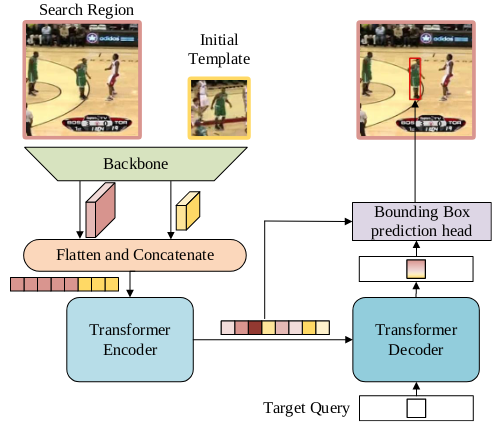
\includegraphics[scale=0.5]{images/stark_base}}
	\caption{
		\begin{footnotesize}
		\textRL{مخطط النموذج الأول من خوارزمية}
		\textLR{STARK}
		\textRL{والذي يستخدم المعلومات المكانية فقط}
		\textLR{\cite{Stark}}
		\end{footnotesize}
	}
	\label{stark_base}	
\end{figure}
للنموذج دخلان هما الـ
\textLR{template}
 من الإطار الأول لعملية الملاحقة 
$Z \in \Re^{{3} \mathsf{x} {H_z} \mathsf{x} W_z}$
حيث 
$H_z = W_z = 128$،
ونافذة البحث 
$X \in \Re^{{3} \mathsf{x} {H_x} \mathsf{x} W_x}$
حيث
$H_x = W_x = 320$.
\subsubsection{المرحلة الأولى - استخلاص السمات}
يتم استخلاص سمات كل من الدخلين عبر 
\textLR{backbone}،
 وهي المراحل الأربعة الأولى من شبكة
\textLR{ResNet\cite{ResNet}}،
فيكون
\textLR{stride}
 الشبكة 
 $s = 16$.
\newline
 خرج الـ
\textLR{backbone}
 هو سمات كل من الـ
\textLR{template}
$f_z \in \Re^{C \mathsf{x} \frac{H_z}{s} \mathsf{x} \frac{W_z}{s}}$،
وسمات نافذة البحث
$f_x \in \Re^{C \mathsf{x} \frac{H_x}{s} \mathsf{x} \frac{W_x}{s}}$.
بعدها  يتم سَلسَلة
\textLR{concatenate}
 سمات الـ
\textLR{template}
وسمات نافذة البحث ضمن سلسلة واحدة، ومن ثم تخفيض أبعاد السلسلة من 
\textLR{C}
إلى
\textLR{d}
، ثم تسطيح 
\textLR{flatten} 
 السلسلة لتصبح بأبعاد
$( d \mathsf{x} \frac{H_z}{s}\frac{W_z}{s} + \frac{H_x}{s}\frac{W_x}{s} )$،
وهذه السلسلة هي دخل المحول.
\subsubsection{المرحلة الثانية - المحول}
%تعتمد بنية المحول في هذه الخوارزمية بشكل كبير على محول  خوارزمية الكشف 
%\textLR{DETR\cite{DETR}}
%مع اختلافات طفيفة مثل عدد
%\textLR{target queries}.
يحتوي المرمز على $6$ طبقات، عدد الرؤوس في تابع الانتباه الذاتي متعدد الرؤوس
$ h=8 $,
أما أبعاد الطبقة المخفية  في شبكات 
\textLR{MLP}
فهي
 $2048$،
الترميز المكاني هو 
\textLR{sinusoidal}
كما في المحول الأصلي.
\newline
هدف  المرمز هو تعديل السمات بحسب السياق وإرسالها إلى مفكك الترميز.
من الشكل
\ref{stark_base}
نلاحظ دخلين لمفكك الترميز
الأول هو خرج المرمز، أما الثاني فهو
\textLR{target query}.
إن بنية المحول في
\textLR{STARK}
تعتمد بشكل كبير على المحول المستخدم في كاشف
\textLR{DETR\cite{DETR}}،
حيث عدد
\textLR{target queries}
هي عدد الأغراض التي يجب الكشف عنها. هنا في 
\textLR{STARK}
كخوارزمية ملاحقة لغرض واحد فإن عدد 
\textLR{target queries = 1}.
 \subsubsection{المرحلة الثالثة - تقدير مكان الهدف }
لتقدير المستطيل المحيط  بالغرض اعتمدت 
\textLR{STARK}
على الكتلة الموضحة في الشكل 
\ref{stark_score_head}
\begin{figure}[!h]
	\centerline{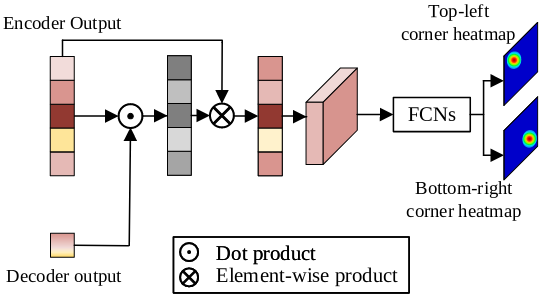
\includegraphics[scale=0.5]{images/stark_score_head}}
	\caption{
		\textRL{شبكة الـ}
		\textLR{regression}
		\textRL{لتقدير مكان الغرض}
		\textLR{\cite{Stark}}}
	\label{stark_score_head}
\end{figure}
هدف هذه الشبكة هو الـ
\textLR{regression}
، أي تقدير إحداثيات  الزاوية العليا اليسارية و الزاوية السفلى اليمينية للمستطيل المحيط.
بداية يحسب التشابه بين خرج المرمز وخرج مفكك الترميز،
 وذلك بحساب الجداء السلمي بينهما. نعدل خرج المرمز بتوزينه بقيم التشابه المحسوب سابقاً، نعدل من شكل خريطة السمات لتصبح ب
 $3$
  أبعاد 
$f \in \Re^{d \mathsf{x} \frac{H_s}{s} \mathsf{x} \frac{W_s}{s}}$.
ونقوم بإدخال خريطة السمات إلى شبكة 
\textLR{FCN}
 مكونة من $ 5$ طبقات تلاففية
\textLR{Conv-BN-ReLU}
 مع تابع تفعيل 
\textLR{ReLU}.
والخرج عبارة عن خريطة احتمالية لزوايا المستطيل المحيط.
\subsubsection{تابع الخطأ}
تابع الخطأ المستخدم في التدريب هو مجموع موزن لتابعين، الأول هو تابع الخطأ 
$L_1$،
والثاني هو
\textLR{GIOU\cite{giou}}
بحسب المعادلة التالية :
\begin{equation}
L = \lambda_{giou} L_{giou}(b_i,\hat{b}_i) + \lambda_{L_1} L_1(b_i,\hat{b}_i)
\label{loss_regression}
\end{equation} 
حيث 
$b_i$
هي القيمة الحقيقية 
\textLR{ground truth}
للمستطيل المحيط، بينما
$\hat{b}_i$
هي القيمة المقدرة (خرج الملاحق)، 
$\lambda_{giou},\lambda_l$
هي
\textLR{hyperparameters}.
\subsection{نموذج 
\textLR{STARK}
الثاني - مع المعلومات المكانية والزمانية}
معظم الملاحقات الحديثة تعتمد فقط على المعلومات المكانية أي معلومات مظهر الهدف وتتجاهل المعلومات الزمنية
\textLR{\cite{swinTrack},\cite{SiamFC}}.
حاولت خوارزمية
\textLR{STARK} 
إدخال المعلومات الزمانية عن طريق دخل ثالث وهو صورة الهدف في آخر عملية ملاحقة، وندعوه بالـ 
\textLR{dynamic template}.
هذا الـ
\textLR{template}
 الجديد الذي يحوي معلومات تغير مظهر الهدف هو ما نعتبره يحمل المعلومات الزمانية، بالإضافة إلى احتفاظ النموذج بالـ
\textLR{template}
الابتدائي.
\newline
يوضح الشكل 
\ref{stark-full}
النسخة الثانية 
(اللون الأحمر) على النسخة الأولية (اللون الأزرق) لخوارزمية 
\textLR{STARK}.
\begin{figure}[!h]
	\centerline{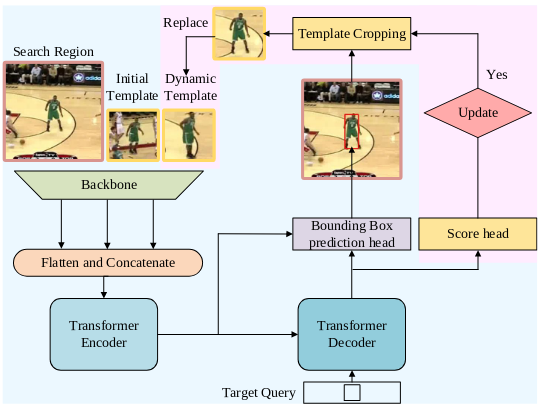
\includegraphics[width=\textwidth]{images/stark_full}}
	\caption{
		\textRL{النسخة الثانية من محول}
		\textLR{STARK}
		\textRL{باستخدام المعلومات الزمانية والمكانية}
		\textLR{\cite{Stark}}}
\label{stark-full}
\end{figure}
وكما في النموذج الأول يتم استخلاص سمات الـ
\textLR{template}
الجديد عبر
\textLR{backbone}،
و تكون مهمة المرمز هي استخلاص السمات المكانية والزمانية من شعاع سمات
 المداخل الثلاثة بعد سَلسَلتها.
\newline
التعديل الثاني في الخوارزمية هو معيار تحديث الهدف،
تم استخدام شبكة
\textLR{score head}
 غرضها التصنيف (هدف أو خلفية)،
% خرجها ندعوه بـ
%\textLR{score}،
يعبر خرجها
(\textLR{score})
 عن احتمالية وجود هدف في الموقع المقابل.
تحتوي الشبكة على ثلاث طبقات
\textLR{MLP}
%نسميها 
%\textLR{score head}،
بُعد الطبقة المخفية $256$، مع تابع تفعيل 
\textLR{sigmoid}.
\newline	
يتم تدريبها بتابع
\textLR{BCE binary cross-entropy}،
بحيث يكون خرج الشبكة
%(\textLR{score})
قيمة عالية عندما تكون وثوقية الهدف أكبر، 
\textRL{ولا يتم التحديث إلا }
عندما تكون هذه القيمة أكبر من حد معين
\textLR{threshold}،
تكون الوثوقية عالية طالما أن نافذة البحث تحوي كامل الهدف.
\newline
لتسهيل عملية تدريب النموذج الكلي
يتم تدريب النموذج على مرحلتين،
المرحلة الأولى يتم تدريب الشبكة بالكامل ماعدا شبكة التصنيف،
%\textLR{score head}،
أي باستخدام تابع الخطأ في المعادلة
\ref{loss_regression}.
المرحلة الثانية هي بتجميد أوزان المرحلة السابقة، وتدريب شبكة التصنيف
%\textLR{score head}
فقط، وذلك باستخدام تابع خطأ
\textLR{BCE}
كما في المعادلة
\ref{BCE}
\begin{equation}
	L_{ce} = log(P_i) + (1-y_i)log(1-P_i)
	\label{BCE}
\end{equation}
حيث
$y_i$
هي القيمة الحقيقة
\textLR{ground truth}،
$Pi$
هي خرج شبكة التصنيف.
\newline
أثناء التدريب يتم اختيار الـ
\textLR{template}
\textRL{الابتدائي}،
الـ
\textLR{template}
الديناميكي
\textRL{ ونافذة البحث}
بشكل عشوائي من
\textRL{القيم الحقيقية}
لمعطيات التدريب
\textRL{لنفس الفيديو}،
بحيث لا يكون البعد بينهما (عدد الإطارات) أكبر من قيمة ندعوها بـ
\textLR{update interval}.
طريقة التدريب هذه استعنّا بها عند تدريب النموذج الخاص بالبحث.
\newline
في مرحلة الملاحقة يتم تحديث الـ
\textLR{template}
 الديناميكي فقط عندما يكون عدد الإطارات بعد آخر تحديث أكبر من  
\textLR{update interval = 200}،
ويكون
$score > 0.5$.
\newline
يبين الجدول 
\ref{table:two_tracker_got10k_results}
نتائج التدريب على مجموعة المعطيات
\textLR{got10k}،
حيث
\textLR{STARK-S50}
 هي النسخة الأولى من الخوارزمية باستخدام المعلومات المكانية فقط، أي دون الـ
\textLR{template}
 الديناميكي، وباستخدام 
\textLR{ResNet50}
 كـ
\textLR{Backbone}.
\newline
\textLR{STARK-ST101}
 هي النسخة الثانية من الخوارزمية، أي باستخدام المعلومات المكانية والزمانية، وباستخدام
\textLR{ResNet101}
 كـ
\textLR{backbone}.
\newline
%****
البنية الصلبة المستخدمة في تدريب واختبار كلا النموذجين هي
\textLR{8 X 16GB Tesla V100 GPU}.
\newline
\textRL{
من الجدول 
\ref{table:two_tracker_got10k_results}
نلاحظ تحسن أداء خوارزمية 
\textLR{STARK}
عند إضافة الـ
\textLR{template}
المحدّث دون 
}
\textRL{
التأثير على سرعة الأداء، مع زيادة طفيفة في حجم النموذج في حال استخدام نفس الـ 
\textLR{backbone}.
}
% \selectlanguage{english}
%\begin{figure}[H]
%	\centering
%	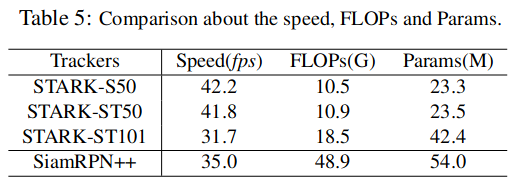
\includegraphics[width=\textwidth]{images/stark_speed}
%	\caption{
%		\cite{Stark}
%		speed of stark
%	}
%\end{figure}
%\selectlanguage{arabic}
\section{\textLR{SwinTrack\cite{swinTrack}}\label{section:swintrack}}
الفكرة الأساسية من البحث هي تعديل ملاحق
\textLR{SwinTrack}
بإدخال المعلومات الزمانية، وذلك بالاستفادة من التعديل المستخدم في ملاحق 
\textLR{STARK}
\ref{section:stark}. 
لذلك سنشرح في هذه الفقرة خوارزمية 
\textLR{SwinTrack}
بشيء من التفصيل، كونها النموذج الأساسي في بحثنا.
\newline
هذا الملاحق يعتمد كلياً على توابع الانتباه لاستخلاص ودمج السمات، إذ أنه يستخدم محول
\textLR{Swin\cite{swintransformer}}
كـ
\textLR{backbone}
لاستخلاص السمات، وبذلك فهو يختلف عن الملاحقات السابقة التي تستخدم المحول كجزء من بنيتها، وتستفيد من شبكات
\textLR{CNN}
%كشبكة
%\textLR{ResNet\cite{ResNet}}
%وشبكة
%\textLR{AlexNet\cite{alexnet}}
لاستخلاص سمات الصور، وذلك كما في خوارزميات الملاحقة
\textLR{Transformer Tracking\cite{transformertracker}}
و
\textLR{STARK\cite{Stark}}.
أما بالنسبة لخوارزمية الملاحقة 
\textLR{SwinTrack}
فهي تستخدم بنية  مرمز- مفكك ترميز
%\textLR{encoder-decoder}
لدمج السمات والتي تعتمد على توابع الانتباه كما في المحول الأصلي
\textLR{\cite{Vaswani17}}. 

\begin{figure}[!h]
	\centerline{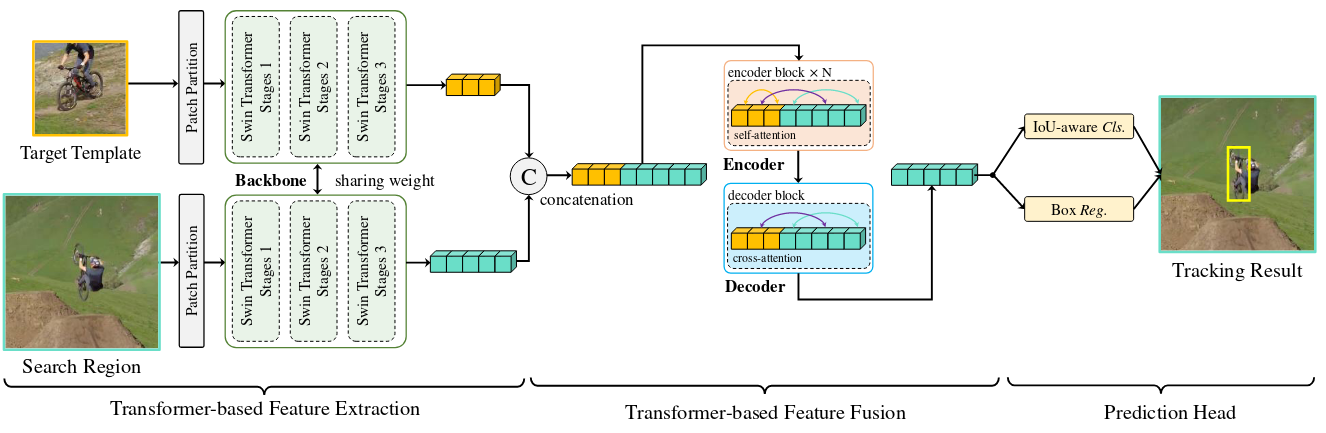
\includegraphics[width=\textwidth]{images/swinTrack}}
	\caption{
		\textRL{بنية الملاحق}
		\textLR{SwinTrack}
		\textLR{\cite{swinTrack}}}
	\label{fig:swintrack}	
\end{figure}
يوضح الشكل 
\ref{fig:swintrack}
مراحل خوارزمية 
\textLR{SwinTrack}،
وهي بشكل أساسي تتكون من ثلاث مراحل، الأولى لاستخلاص السمات، والثانية لدمجها، والثالثة لتحديد مكان وأبعاد الغرض، وسنشرح في الجزء التالي كل مرحلة من هذه المراحل.
\subsection{المرحلة الأولى - استخلاص السمات}
تستخدم هذه الخوارزمية  المراحل الثالث الأولى من محول
\textLR{Swin}
كـ
\textLR{backbone}.
وبمقارنة محول
\textLR{Swin}
بشبكات
\textLR{CNN}
الأخرى
\textLR{\cite{alexnet}\cite{ResNet}}،
 فإن محول
\textLR{Swin}
قادر على إعطاء تمثيل للسمات بشكل أفضل
\textLR{\cite{swintransformer}}.
يوضح الشكل 
\ref{fig:swintrack}
مداخل نموذج الملاحقة 
\textLR{SwinTrack}،
حيث له دخلان الأول هو صورة الـ 
\textLR{template}
الإبتدائي،
والثاني هو نافذة البحث.
\newline
تم تجريب ثلاث نسخ من محول 
\textLR{Swin}
كـ
\textLR{backbone}.
وفيما يلي أبعاد كل نموذج بحسب الـ
\textLR{backbone}
المستخدمة:

\selectlanguage{english}
	\begin{itemize}
		\item SwinTrack-T
		\newline
		Backbone: Swin Transformer-Tiny\cite{swintransformer}
		\newline
		Template size: [112 x 112]; Search region size [224 x 224]; C = 384; N=4
		
		\item SwinTrack-B
		\newline
		Backbone: Swin Transformer-Base\cite{swintransformer}
		\newline
		Template size: [112 x 112]; Search region size [224 x 224]; C = 512; N=8
		
		\item SwinTrack-B-384
		\newline
		Backbone: Swin Transformer-Base\cite{swintransformer}
		\newline
		Template size: [192 x 192]; Search region size [384 x 384]; C = 512; N=8
	\end{itemize}
\selectlanguage{arabic}
حيث $C$ هو بعد النموذج و
$s=16$
هو 
\textLR{stride}
الشبكة،
\textRL{
		و
		$N$
		عدد كتل المرمز
}.
\newline
\subsection{المرحلة الثانية - دمج السمات بالاعتماد على المحول}
يتم سَلسَلة سمات الـ
\textLR{template}
وسمات نافذة البحث ضمن تمثيل موحد $U$ يشكل دخلاً للمرمز.
وكما في المحول الأصلي فإن المرمز يتكون من 
توابع انتباه ذاتي متعددة الرؤوس 
\textLR{MSA}،
مع شبكة عصبونية 
\textLR{FFN}
تتكون من طبقتين مع تابع تفعيل
\textLR{GELU}
\textLR{Gaussian Error Linear Unit}،
مع وجود تنظيم خطي 
\textLR{Linear Normalization}
قبل كل كتلة
\textLR{\textLR{FFN} + MSA}،
و 
\textLR{Residual connection}
 بعد كل كتلة 
\textLR{\textLR{FFN} + MSA}،
وذلك بحسب المعادلات 
\ref{eq:swinencoder}
\begin{equation} \label{eq:swinencoder}
\begin{split}
 &U^1 = Concat(z^1,x^1)\\
 &...\\
 &U^{l^\prime} = U^l + MSA(LN(U^\prime))\\
 &U^{l+1} = U^{l^\prime} + FFN(LN(U^{l^\prime}))\\
 &...\\
 &z^L,x^L = Deconcat(U^L)
\end{split}
\end{equation}


حيث $l$ هي رقم الطبقة، $L$ عدد طبقات المرمز.
كما نرى في آخر معادلة وبحسب الشكل
\ref{fig:swintrack}
فإنه يتم إعادة فصل 
\textLR{deconcatenate}
خرج المرمز وتقسيمه إلى سمات الـ
\textLR{template}
وسمات نافذة البحث.
\newline
يتبع نموذج المحول الأصلي
\textLR{\cite{Vaswani17}}
الطريقة التقليدية في
دمج ومعالجة السمات الآتية من مصادر مختلفة (المصدران في حالتنا هما
\textLR{template}،
ونافذة البحث)، وذلك بحساب الانتباه الذاتي لكل مصدر أي لصورة ال
\textLR{template}
ولصورة نافذة البحث بشكل مستقل، ومن ثم دمج هذه السمات عن طريق 
\textLR{cross-attention}.
هذه الطريقة تدعى بـ
$"$
دمج السمات بالاعتماد على الانتباه التقاطعي
$"$.
%\textRL{بالاعتماد}
% على
%\textLR{cross-attention}$"$.
\newline
أما الطريقة المتبعة في ملاحق
\textLR{Swin}
هي بدمج السمات في دخل المرمز ومعالجتها كسلسلة واحدة، وتسمى بـ
$"$
دمج السمات بالاعتماد على السَلسَلة
\textLR{concatenation-based fusion}
$"$.
وبمقارنة هذه الطريقة بالطريقة السابقة فإنها تخفض التعقيد الحسابي وذلك بانقاص عدد أوزان النموذج، 
\textRL{وبالتالي فهي مناسبة أكثر لتطبيقات الزمن الحقيقي}
\newline
تابع الانتباه هو التابع المستخدم في المحول الأصلي
\textLR{\cite{Vaswani17}}،
إذ لا حاجة لاستخدام تابع انتباه
\textLR{Swin}،
لأن الفرق في التعقيد الحسابي بين التابعين بسيط في حالة دخل صغير الأبعاد، والدخل هنا هو أشعة السمات.
\newline
ترميز الموقع
\textLR{Positional Encoding PE}:
لمساعدة النموذج على تمييز مصادر وأماكن السمات التي تتم معالجتها لابد من إضافة ترميز مكاني إلى السمات، والنوع المستخدم في 
\textLR{SwinTrack}
هو 
\textLR{Untied Positional Encoding\cite{untiedPE}}.
\newline
أما بالنسبة لدخل  مفكك الترميز
 فهو عبارة عن السمات الخارجة من المرمز، وخرجه هو خريطة السمات المعدلة لنافذة البحث
$ x \in \Re^{\frac{H_x}{s} \mathsf{x} \frac{W_x}{s} \mathsf{x} C}$.
تتبع العمليات الحسابية ضمن مفكك الترميز
المعادلات 
\ref{eq2}:
\begin{equation} \label{eq2}
\begin{split}
&U^D = Concat(z^l,x^l)\\
&x^{L^\prime} = x^L + MCA(LN(x^L),LN(U^D))\\
&x = x^{L^\prime} + FFN(LN(x^{L^\prime})).\\
\end{split}
\end{equation}
يحسب تابع الانتباه التقاطعي متعدد الرؤوس
\textLR{MCA}
بين
$x^L$
 خريطة سمات نافذة البحث بعد فك السلسلة، وبين 
$U^D$
%\textLR{Ud}
خرج المرمز والذي يعبر عن سمات كل من الـ
\textLR{template}
ونافذة البحث.
\subsection{المرحلة الثالثة - شبكتي التصنيف وال 
\textLR{regression}
	: }
الخرج النهائي لمفكك الترميز
هو سمات نافذة البحث
$x \in \Re^{\frac{H_x}{s} \mathsf{x} \frac{W_x}{s} \mathsf{x} C}$،
هذه السمات بحاجة إلى معالجة لتحديد موقع الغرض بالنسبة لنافذة البحث.
\newline
يتم استخدام طريقتي التصنيف والـ  
\textLR{regression}
  بشكل منفصل لتحديد موقع الغرض والمستطيل المحيط به.
كل من الكتلتين عبارة عن شبكة عصبونية
\textLR{MLP}
تتكون من ثلاث طبقات، ودخل كل من الشبكتين هو خرج مفكك الترميز.
\newline
الكتلة الأولى هدفها التصنيف ضمن صنفين هما الهدف والخلفية، وخرجها هو خريطة استجابة التصنيف
\textLR{classification response map}
$r_{cls} \in \Re^{(H_x \mathsf{x} W_x) \mathsf{x} 1}$،
بحيث تكون قيمة كل عنصر من عناصر المصفوفة  ضمن المجال
$[0,1]$،
وهذه القيمة تعبر عن احتمالية وجود الغرض في هذا الموقع.
\newline
أما الكتلة الثانية وهي الـ 
\textLR{regression}،
فغايتها التنبؤ بالمستطيل المحيط، وخرجها 
$r_{reg} \in \Re^{(H_x \mathsf{x} W_x) \mathsf{x} 4}$،
كل عنصر من عناصر الخرج يعبر عن إحداثيات الزاوية العليا اليسارية و الزاوية السفلى اليمينية  للمستطيل المحيط.
\newline
%يتم معالجة خرج الشبكتين لتحديد موقع الغرض، فمثلا تم افتراض أن حركة الهدف انسيابية فيتم استخدام 
%\textLR{Hanning penalty}
%للحد من الحركات الكبيرة.
%وفي النهاية
لتحديد موقع الغرض يتم اختيار المستطيل المقابل لأعلى استجابة تصنيف.
وكما لاحظنا من بنية الملاحق فإنه يعتمد بشكل كلي على مظهر الغرض في الإطار الأول للملاحقة دون الأخذ بعين الاعتبار تغيرات شكل الغرض. 
%\textLR{AdamW\cite{AdamW}}
\begin{table}[!h]
	\centering
	\begin{tabular}{c c c c c c c} 
		\hline
		\textLR{Tracker} & $mAO$\% & $mSR_{50\%}$ & $mSR_{75\%}$ &\textLR{Speed($fps$)}&\textLR{FLOPS(G)}&\textLR{Params(M)}\\ [0.5ex] 
		\hline\hline
		\textLR{STARK-S50} &$67.2$&$76.1$&$61.2$&$41.8$&$10.5$&$32.3$\\
		\textLR{STARK-ST50} & $68.0$ & $77.7$ & $62.3$&$41.8$&$10.9$&$32.5$\\ 
		\textLR{STARK-ST101} &$68.8$ & $78.1$ & $64.1$&$31.7$&$18.5$&$42.4$\\
		\hline
		\textLR{SwinTrack-T} & $69.0$ & $78.1$ & $62.1$&$98$&&$23$ \\
		\textLR{SwinTrack-B} & $69.4$ & $78.0$ & $64.3$&$52$&&$91$ \\
		\textLR{SwinTrack-B} &&&&$45$&&$91$\\[1ex] 
		\hline
	\end{tabular}
	\caption{
		\textRL{نتائج خوارزميتي}
		\textLR{SwinTrack,STARK}
		\textRL{من أجل معطيات التدريب}
		\textLR{GOT-10k\cite{got10k}}}
	\label{table:two_tracker_got10k_results}
\end{table}
\newline
%\begin{table}[!h]
%	\centering
%	\begin{tabular}{c c c c c c c} 
%		\hline
%		\textLR{Tracker} & \textLR{AUC}\% & \textLR{Normalized Precision} & \textLR{Precision}&\textLR{Year}\\ [0.5ex] 
%		\hline\hline
%		\textLR{SwinTrack-B-384} &$70.2$&$78.4$&$75.3$&$2021$\\
%		\textLR{STARK} & $67.1$ & $77.0$ &&$2021$\\ 
%		\textLR{TransT} &$64.9$ & $73.8$ & $69.0$&$2021$\\
%		\textLR{TrTr} & $55.1$ &&&$2021$&\\[1ex] 
%		\hline
%	\end{tabular}
%	\caption{
%		\textRL{نتائج خوارزميتي}
%		\textLR{SwinTrack,STARK}
%		\textRL{من أجل معطيات التدريب}
%		\textLR{GOT-10k\cite{got10k}}}
%	\label{table:many_tracker_got10k_results}
%\end{table}

 يوضج الجدول
 \ref{table:two_tracker_got10k_results}
نتائج اختبار خوارزميتي 
\textLR{STRAK\cite{Stark}}
و
\textLR{SwinTrack\cite{swinTrack}}
من أجل مجموعة المعطيات 
\textLR{GOT-10k\cite{got10k}}.
نلاحظ تفوق خوازمية
\textLR{SwinTrack}
في الأداء والسرعة على خوارزمية
\textLR{STARK}.
ونلاحظ أن النسخة
\textLR{SwinTrack-T}
أسرع بمرتين تقريبا من النسخ الأخرى، وهذا ما شجعنا على استخدامها كنموذج أساسي في بحثنا، وتطوير هذه الخوارزمية للحصول على أداء أفضل مع سرعة ملاحقة عالية.
\iffalse
\begin{table}[H]
	\centering
	\begin{tabular}{||p{2.cm}||p{2.cm}||p{2.cm}||p{2.cm}||}
		\hline
		Tracker 	& SwinTrack-Tiny-t4 &\\
		\hline
		SS   		& 79.7 \\
		PS 			& 71.6 \\ 
		NPS 		& 90.1 \\ 
		AO 			& 81.2 \\ 
		SR$_{50\%}$ & 91.1 \\ 
		SR$_{75\%}$ & 79.0 \\
		FPS 		& 66.6\\
		HW 			& NVIDIA GeForce RTX 3060 Laptop GPU\\
		\hline
	\end{tabular}
	\caption{SS : Success Score ,PS : Precision Score , NPS : Normalized Precision Score.
	\newline
	validation}
	\label{table:1}
\end{table}

\label{table:2}
\fi

%
%%report
%\begin{table}[!h]
%	\centering
%	\begin{tabular}{c c c c c c c} 
%		\hline
%		\textLR{Tracker} & $mAO$\% & $mSR_{50\%}$ & $mSR_{75\%}$ &\textLR{Speed($fps$)}&\textLR{FLOPS(G)}&\textLR{Params(M)}\\ [0.5ex] 
%		\hline\hline
%		\textLR{STARK-S50} &$67.2$&$76.1$&$61.2$&$41.8$&$10.5$&$32.3$\\
%		\textLR{STARK-ST50} & $68.0$ & $77.7$ & $62.3$&$41.8$&$10.9$&$32.5$\\ 
%		\textLR{STARK-ST101} &$68.8$ & $78.1$ & $64.1$&$31.7$&$18.5$&$42.4$\\
%		\hline
%		\textLR{SwinTrack-T} & $69.0$ & $78.1$ & $62.1$&$98$&&$23$ \\
%		\textLR{SwinTrack-B} & $69.4$ & $78.0$ & $64.3$&$52$&&$91$ \\
%		\textLR{SwinTrack-B} &&&&$45$&&$91$\\[1ex] 
%		\hline
%	\end{tabular}
%	\caption{
%		\textRL{نتائج خوارزميتي}
%		\textLR{SwinTrack,STARK}
%		\textRL{من أجل معطيات التدريب}
%		\textLR{GOT-10k\cite{got10k}}}
%	\label{table:two_tracker_got10k_results}
%\end{table}
%	
\section{النموذج المقترح\label{section:my_model}}
كما ذكرنا فإن معظم الملاحقات الحديثة تستخدم المعلومات المكانية فقط أي  معلومات مظهر الهدف. كما في 
\textLR{SwinTrack\cite{swinTrack}}
 وغيرها. 
لكن كان هناك بعض المحاولات للاستفادة من المعلومات الزمانية كما في  خوارزمية
\textLR{STARK\cite{Stark}}،
وذلك من خلال إدخال صورة الغرض الجديد الناتج عن الملاحقة كدخل ثالث، كما هو مذكور في الفقرة 
\ref{section:stark}.
\newline
أما في خوارزمية
\textLR{SwinTrack}
والتي هي النموذج الأساسي في بحثنا، فإنها تعتمد فقط على الـ
\textLR{template}
المأخوذ من أول إطار في الملاحقة كدخل أول، ونافذة البحث كدخل ثاني، أي أن التغيرات التي تطرأ على الغرض لا يتم أخذها بعين الاعتبار.
\newline
الفكرة الأساسية من البحث هي الاستفادة من المعلومات الزمانية، كما في ملاحق 
\textLR{STARK\cite{Stark}}،
لتعديل نموذج
\textLR{SwinTrack\cite{swinTrack}}،
وذلك بأخذ صورة الغرض الناتجة عن الملاحقة
و سنسميها
\textLR{dynamic template}
أو الـ
\textLR{template}
الجديد
كدخل ثالث للخوارزمية.
\newline
وكما هو موضح في المخطط 
\ref{fig:my_model}
والذي يوضح التعديل الذي قمنا به على خوارزمية 
\textLR{SwinTrack\cite{swinTrack}}،
 فإن خوارزميتنا تستخرج سمات الـ
\textLR{template}
الجديد
عبر 
\textLR{Swin backbone}،
فيصبح لدينا سمات الـ
\textLR{template}
الابتدائي و سمات الـ
\textLR{template}
الجديد
بحاجة إلى دمج ومعالجة.
\newline 
كان لدينا عدة خيارات لدمج سمات الـ
\textLR{template}
الجديد:
\begin{itemize}
\item
الخيار الأول كما في ملاحق
\textLR{STARK}
وملاحق
\textLR{SwinTrack}
بأن يتم الدمج عن طريق سَلسَلة
\textLR{concatenate} 
سمات الثلاث مداخل في سلسلة واحدة، ونستخدمها كدخل للمرمز لتدريبه على كشف المعلومات الزمانية والمكانية معاً.
\newline
يتطلب هذا الخيار تعديل في عدد أوزان الترميز المكاني 
\textLR{PE}، 
وبالتالي سنضطر لتدريب هذه الأوزان الجديدة مع تدريب كامل النموذج والتي عددها $23$ مليون وزن من أجل نموذج 
\textLR{SwinTrack-T}
\textLR{\cite{swinTrack}}.
وهذا قد يستغرق أكثر من شهر باستخدام وحدة معالجة الرسومات 
\textLR{GPU}
المتوفرة لدينا وهي 
\textLR{NVIDIA GeForce 2080 Ti}،
ومن أجل 
\textLR{epoches = 300}
كما في تدريب النموذج الأصلي على مجموعة معطيات 
\textLR{Got10k\cite{got10k}}.
لذلك وجب التفكير بطريقة ثانية نستفيد من خلالها من أوزان النموذج الأصلي المدرب مسبقاً.
\item 
الخيار الثاني هو دمج وتعديل سمات الـ
\textLR{template}
الابتدائي مع سمات الـ
\textLR{template}
الجديد بطريقة تحافظ على أبعاد دخل المرمز.
\newline
الطريقة المقترحة هنا هي بتطبيق التابع الأساسي في المحول، وهو تابع الانتباه المشروح بشكل مفصل في الفقرة
\ref{section:attention}.
يضمن لنا تابع الانتباه المحافظة على الأبعاد من جهة، ومن جهة أخرى فإن مصفوفات 
$W_K,W_Q,W_V$
يتم تدريبها لتتعلم دمج السمات.
باستخدام هذا التابع تجنبنا تدريب النموذج بالكامل، وركزنا فقط على تدريب تابع الانتباه
\end{itemize}
باختيارنا للخيار الثاني استخدمنا تابع الانتباه التقاطعي باختيار سمات الـ
\textLR{template}
المعدل كـ
\textLR{query}،
واختيار سمات الـ 
\textLR{template}
الابتدائي كـ
\textLR{key}
و
\textLR{value}، 
فيكون دخل المرمز بحسب المعادلات 
\textLR{\ref{eq:MHA}}
\begin{equation}
\begin{split}
&\text{\textLR{MultiHead}}(Q, K, V) = \text{\textLR{Concat}}(head_1,\dots,head_h)W^O\\
&head_i = \text{\textLR{Attention}}(QW_i^Q, KW_i^K, VW_i^V)\\
\end{split}
\label{eq:MHA}
\end{equation}
\newline
حيث 
$i$
هو رقم الرأس في كتلة الانتباه التقاطعي متعدد الرؤوس.
يوضح الشكل 
\ref{fig:my_model}
 التعديل الذي أجريناه في خوارزمية
\textLR{swinTrack}
لدمج المعلومات الزمانية والمكانية.
يتم تعديل الـ
\textLR{ updated template}
بحسب خرج شبكة التصنيف والتي تعبر عن
\textLR{  IOU }
المتنبأ به.
 نختار الـ
 \textLR{template}
 الجديد إذا تحقق
\textRL{شرطان}
 معاً وهما:
 \begin{itemize}
 	\item
 	خرج شبكة التصنيف 
 	%\textLR{IOU-aware classification}
 	أكبر من حد معين
 	\textLR{IOU threshold}
 	\item
 	عدد الإطارات بعد آخر تحديث
	\textLR{update interval}
 	 أكبر من قيمة معينة 
 	وذلك كما في خوارزمية 
 	\textLR{STARK\cite{Stark}}.
 \end{itemize}

\subsection{التدريب}
بما أن النموذج المقترح يستخدم شبكتي تصنيف و
\textLR{regression}
فإنه يحتاج إلى تابعي خطأ مستقلين من أجل عملية التدريب، سنذكر كل منهما في هذه الفقرة.
\subsubsection{تدريب التصنيف}
نستخدم من أجل عملية تدريب شبكة التصنيف تابع الخطأ 
\textLR{varifocal loss\cite{varifocal}}
مع 
\textLR{IOU-aware classification score}،
هذا التابع يستبدل القيمة
$1$ 
من أجل العينات الموجبة (هدف)، والقيمة 
$0$
للعينات السلبية ( خلفية)، بقيمة
\textLR{IOU}
بين المستطيل المحيط المتنبأ به وبين القيمة الحقيقة
\textLR{ground truth}
لمعطيات التدريب
وذلك أثناء عملية التدريب
\textLR{\cite{generalfocalloss},\cite{varifocal}}،
كما توضحه المعادلات 
\ref{eq:vlclass}،
\ref{eq:vlregress}.
\newline
هذا المعيار يدمج تدريب قيمة الـ
\textLR{IOU}
مع تدريب التصنيف، وهو قادر على مساعدة النموذج بالتنبؤ بالمستطيل المحيط بدقة أكبر.
\begin{equation}
VFL(p,q) = \begin{cases}
-q(q\log(p) + (1-q)\log(1-p)) &  q > 0 \\
-\alpha p^\gamma \log(1-p) &  q=0 \\
\end{cases}\\
\label{eq:vlclass}
\end{equation}

\begin{equation} 
\mathbb{L}_{cls} = VFL(p,IOU(b,\hat{b}))
\label{eq:vlregress}
\end{equation}

حيث
$q$ 
هي قيمة
\textLR{IOU}
، و
$p$
هي خرج شبكة التصنيف تعبر عن احتمالية وجود الغرض، 
$b$:
المستطيل المحيط المتنبأ به،
$\hat{b}$:
المستطيل المحيط الحقيقي في معطيات التدريب
\textLR{ground truth}.
\newline
\subsubsection{تدريب الـ
\textLR{regression}}
من أجل تدريب شبكة الـ
\textLR{regression}
نستخدم تابع الخطأ
\textLR{Generalized IOU\cite{giou}}
بحسب المعادلة
\textLR{\ref{eq:giou}}
\begin{equation} 
\mathbb{L}_{reg} =\sum_{j} \mathds{1}_{q > 0} [p\mathbb{L}_{GIOU}(b_j,\hat{b})]
\label{eq:giou}
\end{equation}
وذلك فقط من أجل
$IOU=q>0$،
أي يتم تجاهل العينات السلبية التي تمثل الخلفية أثناء التدريب، ويتم إعطاء أهمية أكبر للعينات ذات الاحتمالية العالية
وذلك بتوزين تابع الخطأ 
\textLR{GIOU}.
\newline
وكما في خوارزمية 
\textLR{STARK}
فإنه يتم استخدام تابع خطأ مكون من مجموع موزن لتابعي الخطأ السابقين لتدريب النموذج الكلي.
يتم تحديد أوزان النموذج باستخدام خوارزمية الأمثلة
\textLR{AdamW\cite{AdamW}}.
\begin{figure}[!h]
	\centerline{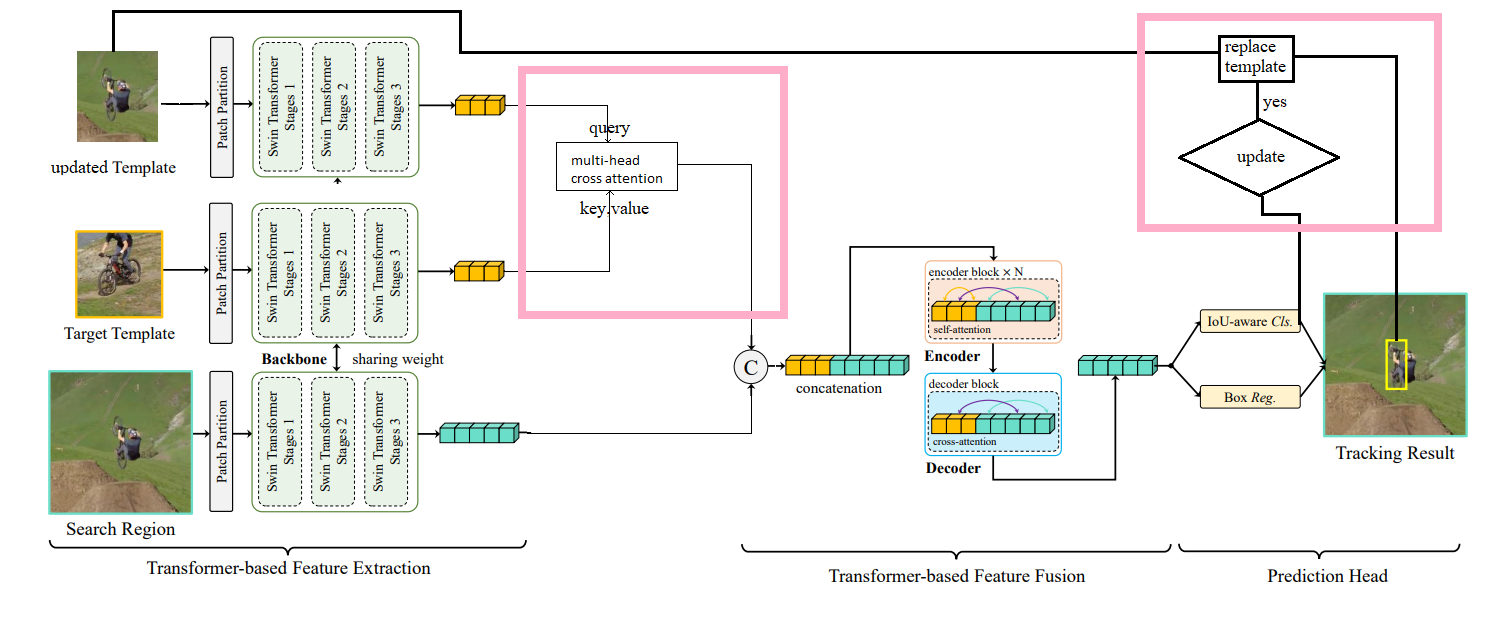
\includegraphics[width=\textwidth]{images/my_model}}
	\caption{\textRL{بنية النموذج المقترح والذي يقوم بدمج سمات صورتي الغرض عبر كتلة انتباه}}
	\label{fig:my_model}
\end{figure}
\section{خاتمة}
تحدثنا في هذا الفصل عن النموذج الأساسي في بحثنا وهو
\textLR{swinTrack}،
وبينا أن مشكلته اعتماده فقط على المعلومات المكانية، بالرغم من سرعته وتفوقه في الأداء على كثير من الملاحقات.   اعتمدنا عندها على طريقة خوارزمية
\textLR{STARK}
في إدخال المعلومات الزمانية. لذلك اقترحنا نموذج يستفيد من معلومات تغير المظهر كمعلومات زمانية، دون تغيير في بنية النموذج الأصلي، للاستفادة من أوزانه في عملية التدريب. وبما أن هذا التعديل قد حسن من أداء 
\textLR{STARK}
فقد توقعنا في بداية مرحلة البحث أنه سيحسن أداء 
\textLR{SwinTrack}.
